\documentclass[slovak]{article}
\usepackage[dvips]{graphicx}        % to include images
\usepackage{pslatex}	    % to use PostScript fonts
\usepackage[T1]{fontenc}
\usepackage[utf8]{inputenc}
\usepackage{pslatex}

\usepackage{tabularx} % tabulky na celu sirku strany
\usepackage{graphicx} %graphics files inclusion
\usepackage{longtable}
\usepackage{multirow}
\usepackage{mathtools}
\usepackage{listings}
\usepackage{listings}
\usepackage{pdfpages}
\usepackage{amsmath}
\usepackage{lscape}

\hyphenation{re-fe-ren-čné}
\hyphenation{de-kom-po-zí-cie}
\hyphenation{ma-xi-mál-ny}
\hyphenation{ma-xi-mál-na}
\hyphenation{al-go-rit-mus}
\hyphenation{e-xakt-né-mu}
\hyphenation{in-štan-cie}
\hyphenation{na-me-ra-ných}
\hyphenation{us-po-ria-da-ní}

\begin{document}

\title{Problém batohu - 4. úloha \\[5mm] MI-PAA, zimný semester 2014}
\author{Martin Klepáč}
\date{\today}

\maketitle

\section{Definícia problému}

Problém batohu (knapsack problem) je jeden z NP-ťažkých problémov. Pokiaľ máme k dispozícii množinu predmetov, pričom každý predmet má svoju váhu, cenu, a maximálnu nosnosť batohu, potom je naším cieľom vybrať predmety do batohu tak, aby sme maximalizovali ich cenu a pritom celková hmotnosť predmetov nepresiahla maximálnu povolenú nosnosť batohu.

\section{Formát vstupu}

Formálne, vstup vyjadríme pomocou

\begin{itemize}

\item \emph{n} = počet predmetov

\item \emph{M} = maximálna nosnosť batohu

\item \emph{vektor w} = hmotnosť jednotlivých predmetov

\item \emph{vektor c} = hodnota (cena) jednotlivých predmetov

\end{itemize}

Výstupom algoritmu je vektor \emph{x}, ktorý udáva prítomnosť/neprítomnosť daného predmetu vo výbere. Ďalej požadujeme informáciu o celkovej hmotnosti predmetov v batohu a ich súhrnú hodnotu pre najlepší výber.


\section{Úvod}

V poslednej úlohe venovanej problému batohu je cieľom otestovať si nasadenie algoritmu simulovaného ochladzovania respektíve genetického algoritmu na tento problém. Okrem samotnej implementácie je potrebné experimentálne zhodnotiť výkonnosť algoritmu pri zmene parametrov.

\section{Simulované ochladzovanie}

Pre túto úlohu som si vybral algoritmus simulovaného ochladzovania, ktorý mi pripadá jednoduchší na pochopenie. Simulované ochladzovanie predstavuje lokálnu metódu prehľadávania stavového priestoru. Metóda umožňuje s určitou pravdepodobnosťou prijať aj stav horší od aktuálneho stavu, ale táto pravdepodobnosť klesá s postupným ochladzovaním, čo v konečnom dôsledku zaisťuje konvergenciu algoritmu. Pseudokód metódy vyzerá nasledovne:

\begin{lstlisting}

function simulatedAnnealing ()
{
  current_temp = INITIAL_TEMP;
  state = INITIAL_STATE;
  while (current_temp > LOWER_BOUND_TEMP)
  {
    steps = NO_OF_STEPS;
    while (steps > 0)
    {
      state = newState (state, current_temp);
      if (state > bestState)
      {
        bestState = state;
      }
      steps--;
    }
    current_temp = cool (current_temp)
  }
}

\end{lstlisting}

\emph{Cool} je funkcia, ktorá zníži aktuálnu teplotu aplikovaním koeficientu ochladzovania \emph{COOLING\_FACTOR}. \emph{NewState} je funkcia, ktorá vracia nejaký nový stav, pričom pravdepodobnosť, že funkcia vráti horší stav ako aktuálny klesá s poklesom aktuálnej teploty \emph{current\_temp}. Jej implementácia je zhodná so slidom číslo 13 prednášky číslo 8 - Simulované ochlazování. Výstupom algoritmu je \emph{bestState} - najlepší nájdený výber.

\section{Výsledky}

Merania prebiehali na 64-bitovom Linuxovom hostiteľovi použitom v predchádzajúcich úlohách. Pre potreby vyladenia algoritmu som experimentálne zisťoval hodnoty počiatočnej a koncovej teploty (v pseudokóde vyššie označené ako \emph{INITIAL\_TEMP} resp. \emph{LOWER\_BOUND\_TEMP}), ďalej koeficient ochladzovania \emph{COOLING\_FACTOR} a počet iterácií vnútorného cyklu - \emph{NO\_OF\_STEPS}. 

Merania prebiehali iteratívne, čo znamená, že najskôr som zmeral závislosť doby behu algoritmu a priemernej/maximálnej relatívnej chyby v závislosti od variabilného koeficientu ochladzovania (ostatné premenné zostali zafixované s určitými hodnotami). Následne som z výsledkov odhadol optimálny koeficient ochladzovania a začal študovať závislosť od počiatočnej teploty. K tomu bolo potrebné zafixovať ostatné premenné na určitých hodnotách s tým, že optimálny koeficient ochladzovania som už mal experimentálne zistený. Takto som vždy jednou sadou merania zistil optimálnu hodnotu ďalšieho parametru. Konečne, po zistení optimálnych hodnôt všetkých parametrov som všetky experimenty vykonal ešte raz - jednu premennú som menil a všetky ostatné boli zafixované s použítím zisteného optima. Výsledky pre veľkosť inštancie \emph{n=40} uvádzam v tabuľkách \ref{tab1} až \ref{tab4} resp. v grafoch \ref{gr:graf1} až \ref{gr:graf4}. Graf \ref{gr:graf5} zobrazuje závislosť ceny riešenia od aktuálneho čísla iterácie pre jednú konkrétnu inštanciu zo vzorky inštancií pre n=40. 

\begin{table}[htb!]\centering
	\begin{tabularx}{\textwidth}{ | X | X | X | X |}
	  \hline                       
		\textbf{Koeficient ochladzovania}	& \textbf{Doba behu [s]} 	& \textbf{Priem. rel. chyba [\%]} 	& \textbf{Max. rel. chyba [\%]} 	\\ \hline
		\textbf{c=0.800}	&	0.012 644	&	0.111	&	2.3372	\\ \hline
		\textbf{c=0.825}	&	0.014 974	&	0.088 	&	2.3372	\\ \hline
		\textbf{c=0.850}	&	0.018 121	&	0.058	&	2.3372	\\ \hline
		\textbf{c=0.875}	&	0.021 101	&	0.048	&	2.3372	\\ \hline
		\textbf{c=0.900}	&	0.026 915	&	0.058	&	2.3372	\\ \hline
		\textbf{c=0.925}	&	0.037 111	&	0.054	&	2.3372	\\ \hline
		\textbf{c=0.950}	&	0.055 780	&	0.047	&	2.3372	\\ \hline
		\textbf{c=0.975}	&	0.110 550	&	0.052	&	2.3372	\\ \hline
	\end{tabularx}
\caption{Závislosť trvania doby behu a relatívnej chyby simulovaného ochladzovania od koeficientu ochladzovania}
\label{tab1}
\end{table}

\begin{table}[htb!]\centering
	\begin{tabularx}{\textwidth}{ | X | X | X | X |}
	  \hline                       
		\textbf{Počiatočná teplota}	& \textbf{Doba behu [s]} 	& \textbf{Priem. rel. chyba [\%]} 	& \textbf{Max. rel. chyba [\%]} 	\\ \hline
		\textbf{t=50}	&	0.009 352	&	0.103	&	2.3372	\\ \hline
		\textbf{t=100}	&	0.011 937	&	0.063 	&	2.3372	\\ \hline
		\textbf{t=200}	&	0.014 823	&	0.068	&	2.3372	\\ \hline
		\textbf{t=400}	&	0.017 581	&	0.058	&	2.3372	\\ \hline
		\textbf{t=700}	&	0.020 288	&	0.072	&	2.3372	\\ \hline
		\textbf{t=1 000}	&	0.021 640	&	0.084	&	2.3372	\\ \hline
		\textbf{t=1 500}	&	0.024 060	&	0.082	&	2.3372	\\ \hline
		\textbf{t=2 000}	&	0.023 636	&	0.087	&	2.3372	\\ \hline
		\textbf{t=3 000}	&	0.025 271	&	0.072	&	2.3372	\\ \hline
		\textbf{t=5 000}	&	0.027 588	&	0.097	&	2.3372	\\ \hline
	\end{tabularx}
\caption{Závislosť trvania doby behu a relatívnej chyby simulovaného ochladzovania od počiatočnej teploty}
\label{tab2}
\end{table}

\begin{table}[htb!]\centering
	\begin{tabularx}{\textwidth}{ | X | X | X | X |}
	  \hline                       
		\textbf{Konečná teplota}	& \textbf{Doba behu [s]} 	& \textbf{Priem. rel. chyba [\%]} 	& \textbf{Max. rel. chyba [\%]} 	\\ \hline
		\textbf{t=0.5}	&	0.025 798	&	0.062	&	2.3372	\\ \hline
		\textbf{t=1}	&	0.023 568	&	0.088 	&	2.3372	\\ \hline
		\textbf{t=2}	&	0.022 017	&	0.078	&	2.3372	\\ \hline
		\textbf{t=5}	&	0.017 258	&	0.058	&	2.3372	\\ \hline
		\textbf{t=10}	&	0.014 903	&	0.105	&	4.8414	\\ \hline
		\textbf{t=20}	&	0.012 658	&	0.246	&	9.8497	\\ \hline
	\end{tabularx}
\caption{Závislosť trvania doby behu a relatívnej chyby simulovaného ochladzovania od konečnej teploty}
\label{tab3}
\end{table}

\begin{table}[htb!]\centering
	\begin{tabularx}{\textwidth}{ | X | X | X | X |}
	  \hline                       
		\textbf{Počet iterácií}	& \textbf{Doba behu [s]} 	& \textbf{Priem. rel. chyba [\%]} 	& \textbf{Max. rel. chyba [\%]} 	\\ \hline
		\textbf{no=100}			&	0.000 197 	&	2.501	&	5.4936	\\ \hline
		\textbf{no=1 000}		&	0.001 773	&	0.535 	&	3.7279	\\ \hline
		\textbf{no=10 000}		&	0.017 543	&	0.058	&	2.3372	\\ \hline
		\textbf{no=100 000}		&	0.175 100	&	0.046	&	2.3372	\\ \hline
		\textbf{no=1 000 000}	&	1.676 700	&	0.046	&	2.3372	\\ \hline
	\end{tabularx}
\caption{Závislosť trvania doby behu a relatívnej chyby simulovaného ochladzovania od počtu iterácií}
\label{tab4}
\end{table}

\begin{figure}[htb!]\centering
	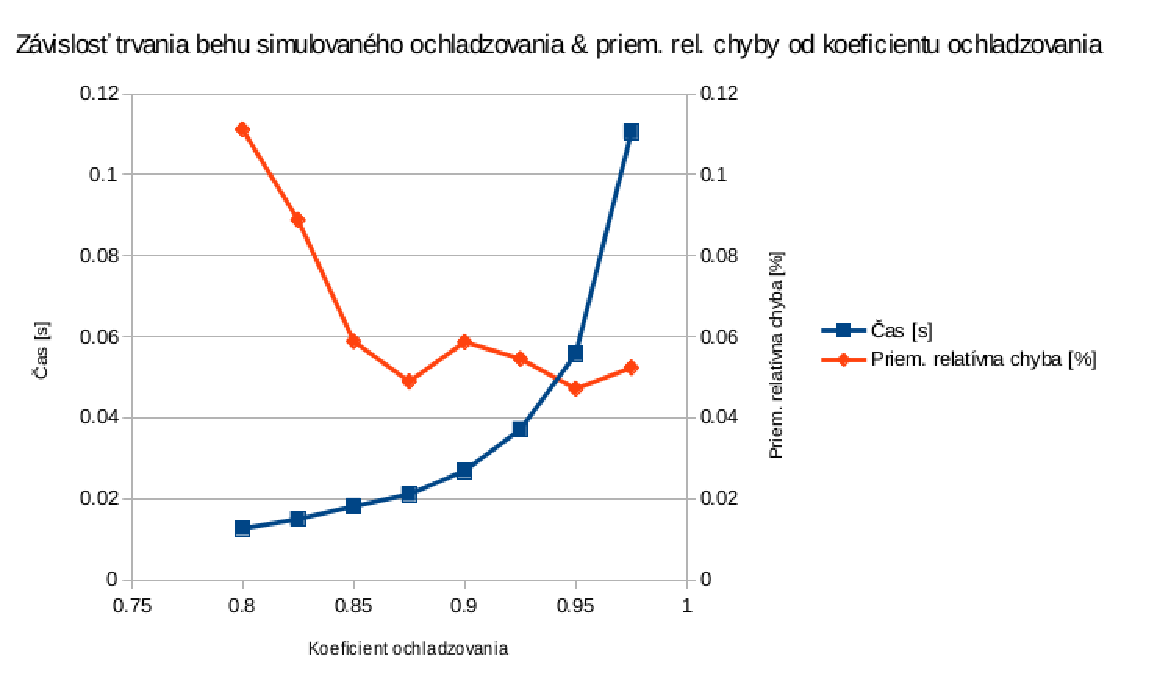
\includegraphics[scale=0.8]{./4_1.pdf}
	\caption{Závislosť trvania doby behu a relatívnej chyby simulovaného ochladzovania od koeficientu ochladzovania}
	\label{gr:graf1}
\end{figure}

\begin{figure}[htb!]\centering
	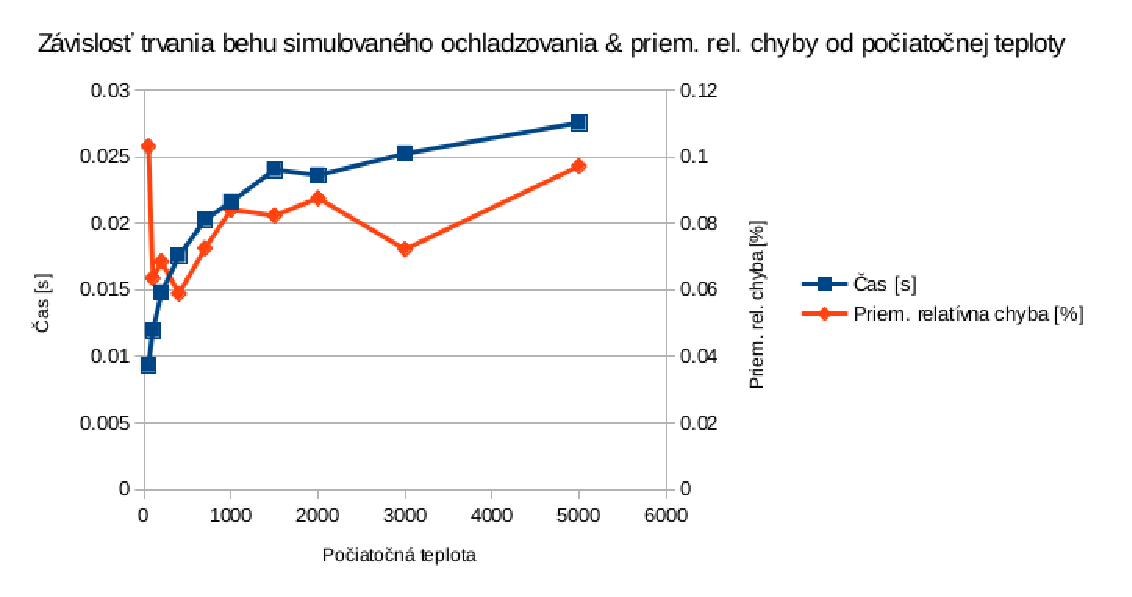
\includegraphics[scale=0.8]{./4_2.pdf}
	\caption{Závislosť trvania doby behu a relatívnej chyby simulovaného ochladzovania od počiatočnej teploty}
	\label{gr:graf2}
\end{figure}

\begin{figure}[htb!]\centering
	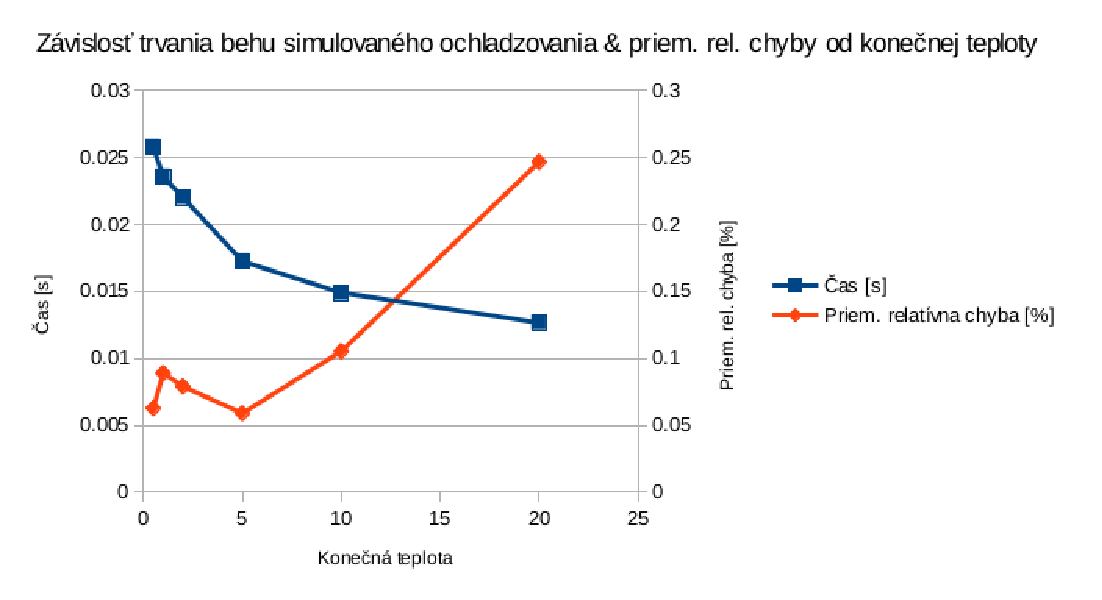
\includegraphics[scale=0.8]{./4_3.pdf}
	\caption{Závislosť trvania doby behu a relatívnej chyby simulovaného ochladzovania od konečnej teploty}
	\label{gr:graf3}
\end{figure}

\begin{figure}[htb!]\centering
	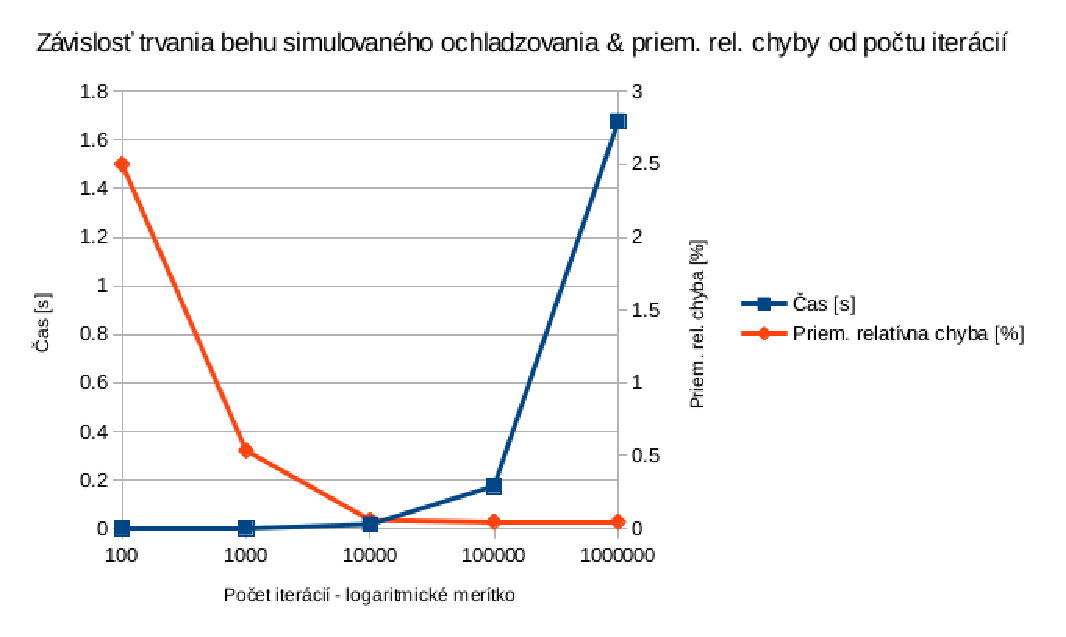
\includegraphics[scale=0.8]{./4_4.pdf}
	\caption{Závislosť trvania doby behu a relatívnej chyby simulovaného ochladzovania od počtu iterácií}
	\label{gr:graf4}
\end{figure}

\begin{figure}[htb!]\centering
	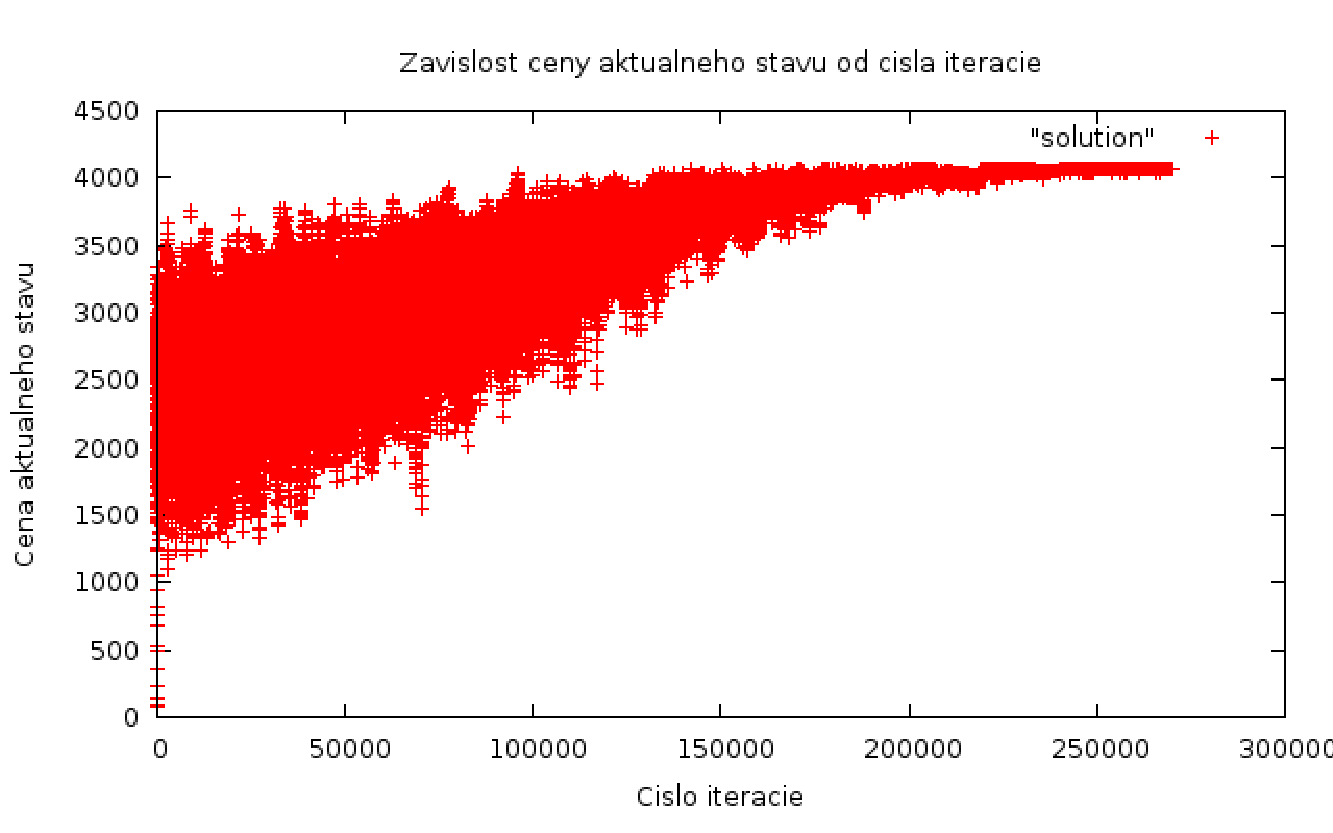
\includegraphics[scale=0.6]{./4_5.pdf}
	\caption{Závislosť ceny aktuálneho stavu od čísla iterácie}
	\label{gr:graf5}
\end{figure}

\section{Zhodnotenie}

Pomocou metodiky v sekcii Výsledky som dospel k nasledovným optimálnym hodnotám parametrov:
\begin{itemize}
  \item INITIAL\_TEMP = 400
  \item LOWER\_BOUND\_TEMP = 5
  \item COOLING\_FACTOR = 0.85
  \item NO\_OF\_STEPS = 10 000
\end{itemize}

Obecne, otázku určenia optimálnych hodnôt jednotlivých parametrov môžeme preformulovať nasledovne - v prípade, ak algoritmus simulovaného ochladzovania necháme bežať dlhšie, o koľko dôjde k zmenšeniu relatívnych chýb v porovnaní s exaktnými riešeniami, akým je napríklad algoritmus dynamického programovania? 

Ukázalo sa, že vysoký chladiaci pomer, nad 0.9 (=pomalé chladenie) výrazným spôsobom neznižuje relatívne chyby v porovnaní s optimálnou hodnotou 0.85.

Z hľadiska počiatočnej teploty sa ako optimálne ukázali byť hodnoty okolo 500. Pre testované inštancie o veľkosti \emph{n=40} dosahovala najlepší pomer relatívnej chyby k dobe behu algoritmu teplota t=400, pre inú veľkosť inštancií sa ako optimálna počiatočná teplota ukázala byť hodnota 700.

Ďalej, s narastajúcou konečnou teplotou klesala na rozdiel od dvojice predchádzajúcich premenných doba behu algoritmu a zároveň dochádzalo k nárastu relatívnych chýb.  Ako optimálnym riešením sa zdá byť hodnota konečnej teploty rovná 5, pri ktorej algoritmus dosahoval najmenšiu relatívnu chybu so zachovaním rozumnej doby behu.

Konečne, s narastajúcim počtom iterácií vnútorného cyklu, dochádza k rádovému rastu doby behu algoritmu pri mojich testovaných hodnotách. Rozumný pomer dosahovali hodnoty 1 000 a 10 000 iterácií. Pre otestovanie dostatočného počtu stavov som za optimálnu zvolil vyššiu hodnotu, t.j. 10 000 iterácií.  

Pri týchto optimálnych hodnotách dosahuje priemerná relatívna chyba 0.058 percenta, maximálna relatívna chyba 2.33 percenta pre vzorky inštancií n=40.

\end{document}
